\documentclass[nobib]{tufte-handout}

\title{Privacy Tools for Data Sharing}

\author[Stephen Weis]{Stephen Weis}

%\date{28 March 2010} % without \date command, current date is supplied

%\geometry{showframe} % display margins for debugging page layout

\usepackage{graphicx} % allow embedded images
  \setkeys{Gin}{width=\linewidth,totalheight=\textheight,keepaspectratio}
  \graphicspath{{graphics/}} % set of paths to search for images
\usepackage{amsmath}  % extended mathematics
\usepackage{booktabs} % book-quality tables
\usepackage{units}    % non-stacked fractions and better unit spacing
\usepackage{multicol} % multiple column layout facilities
\usepackage{lipsum}   % filler text
\usepackage{fancyvrb} % extended verbatim environments
  \fvset{fontsize=\normalsize}% default font size for fancy-verbatim environments

% Standardize command font styles and environments
\newcommand{\doccmd}[1]{\texttt{\textbackslash#1}}% command name -- adds backslash automatically
\newcommand{\docopt}[1]{\ensuremath{\langle}\textrm{\textit{#1}}\ensuremath{\rangle}}% optional command argument
\newcommand{\docarg}[1]{\textrm{\textit{#1}}}% (required) command argument
\newcommand{\docenv}[1]{\textsf{#1}}% environment name
\newcommand{\docpkg}[1]{\texttt{#1}}% package name
\newcommand{\doccls}[1]{\texttt{#1}}% document class name
\newcommand{\docclsopt}[1]{\texttt{#1}}% document class option name
\newenvironment{docspec}{\begin{quote}\noindent}{\end{quote}}% command specification environment

\begin{document}

\maketitle% this prints the handout title, author, and date

 \begin{abstract} \noindent This is an overview of common tools and definitions
for anonymizing data or privately computing with othe parties. It is roughly in
order of practicality and maturity. \end{abstract}

\section{Lossy Techniques} \textbf{Minimization} refers to collecting only the
minimal data necessary for a specific purpose. \textbf{Redaction} deletes or
censors data which has already been collected.

%\begin{marginfigure} 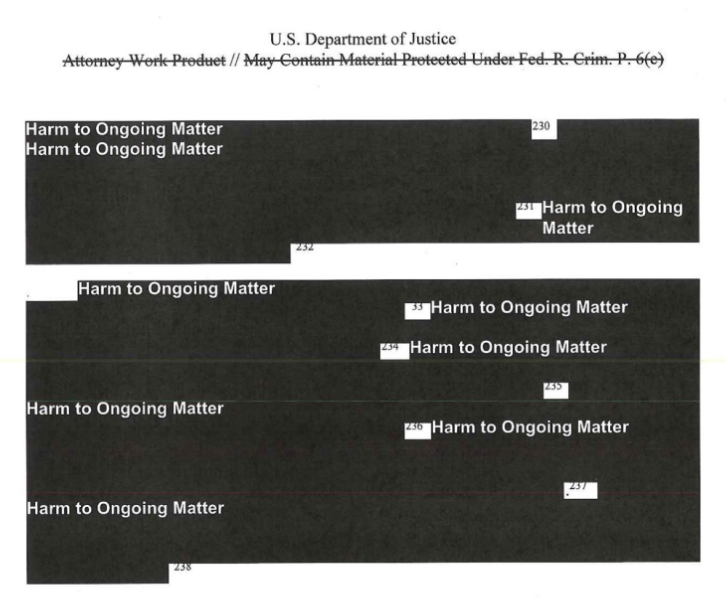
\includegraphics[width=\linewidth]{redacted}
%\caption{Redaction is heavily used in government and legal documents.}
%\label{fig:binned} \end{marginfigure}


\textbf{Aggregation} transforms a set of individual values to reduced set of
values. Summing or averaging are the most common aggregation operations.
Training machine learning models or projecting high-dimensional data to lower
dimensions are also forms of aggregation.

One concern with aggregation are \textbf{differencing attacks} which compare two
aggregated values for different sets and extract the individual input values.
For example, given the average of Alice and Bob’s salary and the average of
Alice, Bob, and Carol’s salary, you can learn Carol’s salary.

\textbf{Generalization} reduces distinguishing values to to more general values
while attempting to maintain utility. This includes both quantitative values
like times or locations as well as qualitative values like names.
\textbf{Binning} or \textbf{bucketing} generalizes quantitative values to
buckets or ranges through rounding or truncation. Common examples are
truncating GPS coordinates to 3 decimal places or rounding time values to the
nearest 15 minute period.

\begin{marginfigure} 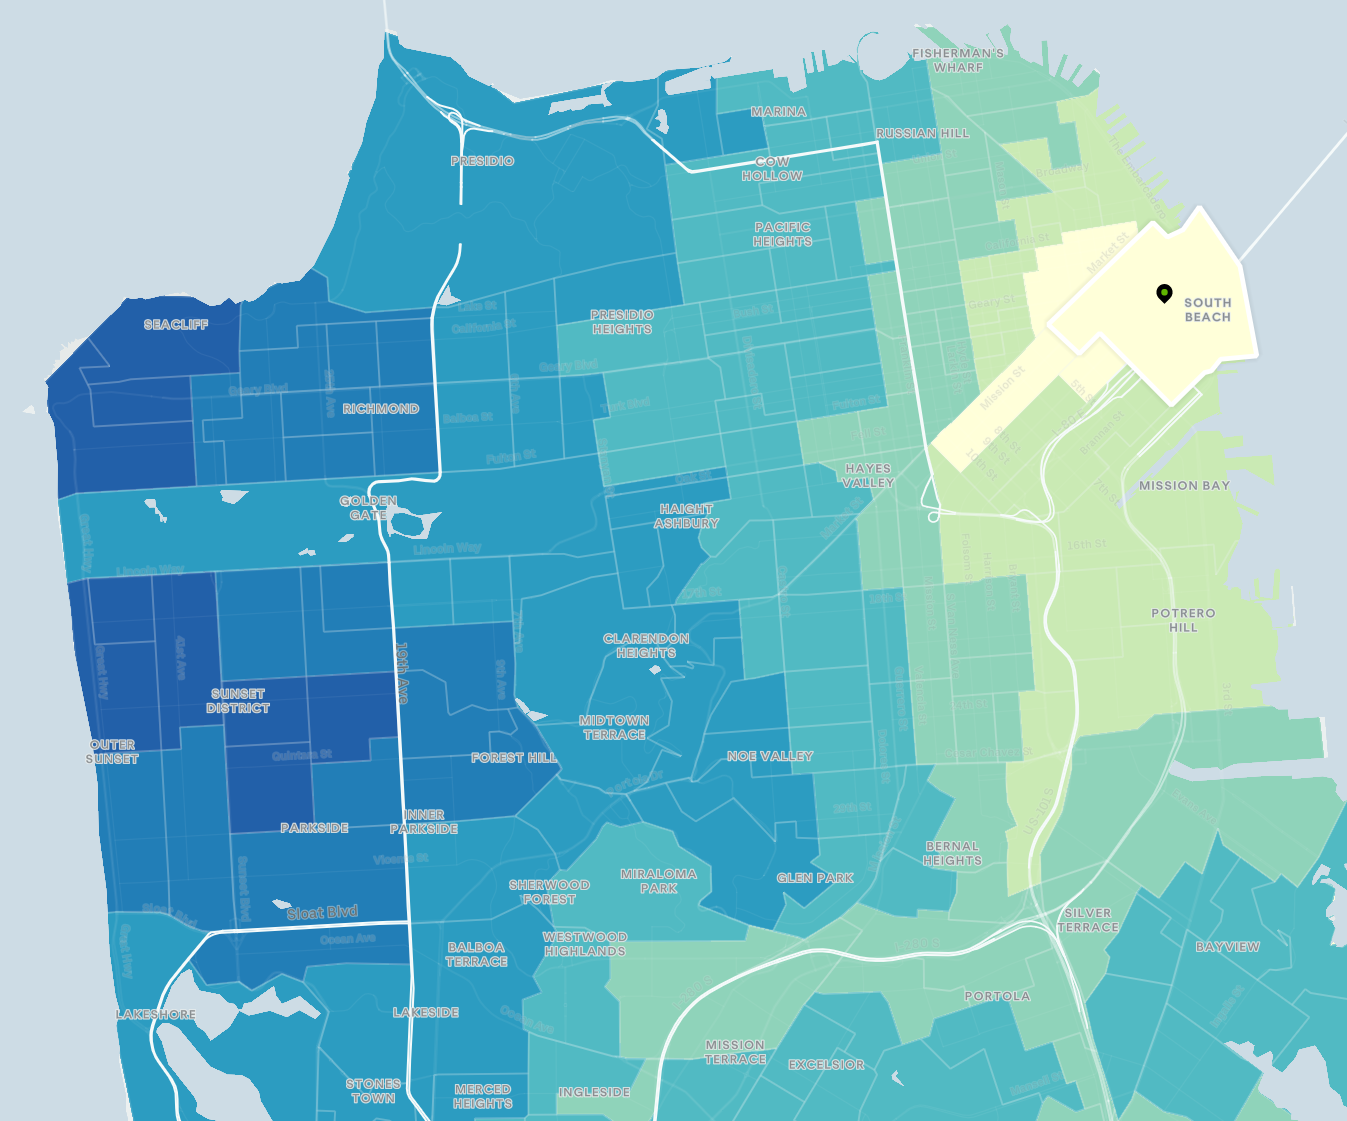
\includegraphics[width=\linewidth]{binned}
\caption{An example map of aggregated geolocation data, binned by neighborhood
and time.}
\label{fig:binned} \end{marginfigure}


\section{k-Anonymity and Extensions}

Implicit in binning values for privacy is the notion of safety in numbers --
that an individuals’ data will be grouped with others in the same bin and that
they will have plausible deniability. The notion of \textbf{$k$-anonymity}
\cite{DBLP:journals/ijufks/Sweene02} is that at least $k$ people will be in any
given bin or group. Aggregated data, APIs, or visualization tools often have
minimum thresholds before returning any data, so are $k$-anonymous in practice.
Google often uses $k$ values of 1000 in their ads and analytics
products. Facebook has used it as low as 20 for ads products.

$K$-anonymity has some privacy issues in practice. First, some bins of data may be
homogenous and all share sensitive traits. For example, a $k$-anonymous set of
geolocations around a specific health clinic might imply health status for that
entire group. A second problem is that background knowledge can be joined to a
k-anonymous data set and be used to deanonymize people.

\textbf{L-diversity} \cite{DBLP:conf/icde/MachanavajjhalaGKV06} is an extension
of $k$-anonymity that addresses the homogeneity issue by ensuring that sensitive
traits among bin have at least $l$ distinct values. \textbf{$T$-closeness}
\cite{DBLP:conf/icde/LiLV07} is a further refinement that ensures that those
distinct values are distributed similarly to the population that data are drawn
from. Neither $l$-diversity nor $t$-closeness have wide adoption in practice,
though Google offers an $l$-diversity measurment in their data loss pervention
API \cite{google-risk-analysis}.

Pseudonymization and Tokenization \textbf{Pseudonymization} or
\textbf{tokenization} means replacing sensitive values like names, credit card
numbers, or phone numbers with surrogate or token values. These tokens retain
their original relationship in the data set and are often used as database
lookup keys.

Tokenization often uses a \textbf{lookup table with random values} mapping to
original values. This has the strongest security guarantee, but requires storing
an entire table of the original data.

\textbf{Pseudorandom functions} (PRFs) are functions which take a secret key as
input whose output is indistinguishable from randomness. PRFs have similar
security properties as random lookup tables, but without having to store the
relationship. HMACs like HMAC-SHA256 are often used as PRFs in practice.

\textbf{Format preserving encryption} \cite{DBLP:conf/sacrypt/BellareRRS09}
(FPE) entails encrypting sensitive fields such that the output ciphertext has
the same format as the input. For example, an format-preserving encrypted credit
card would have 16 decimal digits. AES FFX mode \cite{dworkin2016recommendation}
is one recent standard for FPE encryption.

\begin{marginfigure}
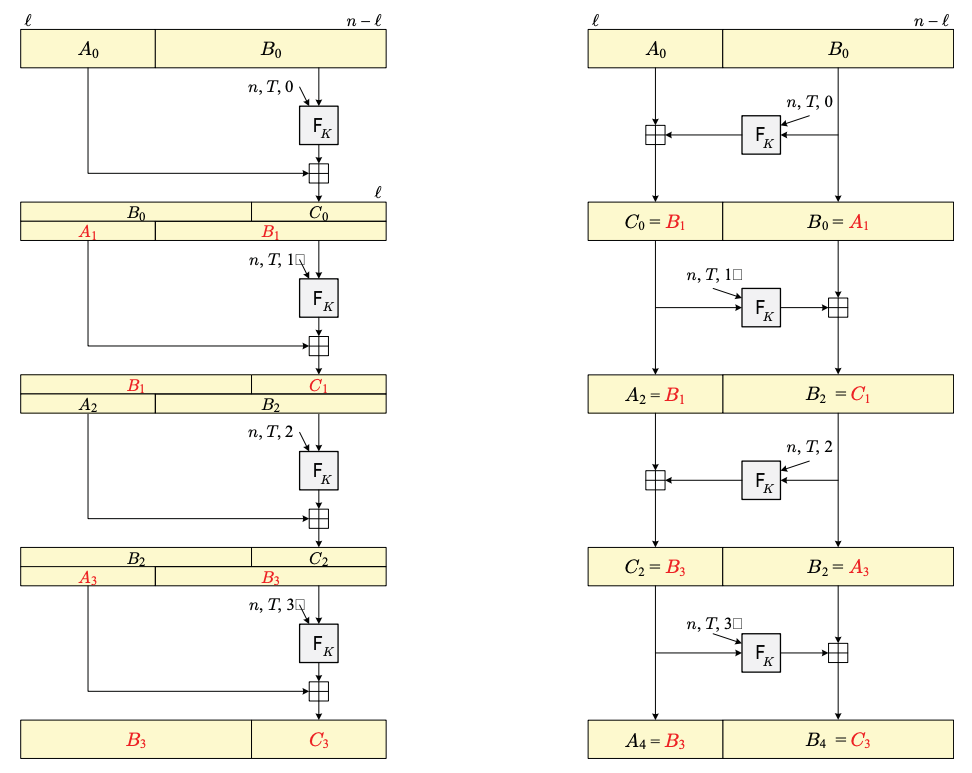
\includegraphics[width=\linewidth]{ffx}
\caption{Illustration of the FFX format preserving encryption mode} \label{fig:ffx}
\end{marginfigure}

Historically, \textbf{one-way functions} have often been misused for
pseudonymization. Many examples of re-identification have occurred when someone
naively used a hash function like MD5 or SHA-1 and stored the digests without
salting the input. Hash functions are not keyed like PRFs. Rather, anyone can
compute them.

The risk of unkeyed hash functions is if the input values have low entropy or
are from a known set. That allows someone to conduct a \textbf{dictionary
attack} where they simple try hashing many values or use precomputed known hash
values available online. Developers often try to avoid this by including an ad
hoc salt value. In general, simply hashing should be avoided unless the input is
known to be high-entropy.

\section{Differential Privacy}

\textbf{Differential privacy} defines the amount of information about an
individual which could be leaked from a dataset. Differential privacy is used by
the US Census \cite{census-differential-privacy}, Apple
\cite{apple-differential-privacy}, Google \cite{google-differential-privacy},
Facebook \cite{facebook-url-release}, and Uber \cite{uber-differential-privacy}
to protect research and user data. Fundamentally, achieving differential privacy
means adding some form of noise or randomization while sacrificing accuracy. In
its most basic form, differential privacy specifies a numerical bound,
$\epsilon$, on how much an algorithm’s output can change between two neighboring
datasets that only differ in a single element. Part of the value of differential
privacy is that $\epsilon$-private systems can be composed with easily
understood properties. This lets one set a privacy budget and allow queries
until that budget is exhausted.

A \textbf{privacy mechanism} is an implementation that achieves some target
$\epsilon$-privacy. A simple mechanism is randomized response, which was
designed to allow people to answer surveys about sensitive topics. The idea is
that you flip a coin Heads to either answer honestly (e.g. \textit{“Did you
cheat on your taxes?”}) or Tails to commit to the answer with negative
connotations (\textit{“Yes”}). This gives the survey taker plausible deniability
that they simply flipped a Tails. It is also easy to account for the noise and
estimate the true answer rate.

Another basic mechanism is the \textbf{Laplace Mechanism}, which adds randomly
sampled noise from the Laplace distribution. This is a simple mechanism that is
tunable to achieve any chosen level of $\epsilon$-privacy and does not depend on
the domain of the input data.

\begin{marginfigure} 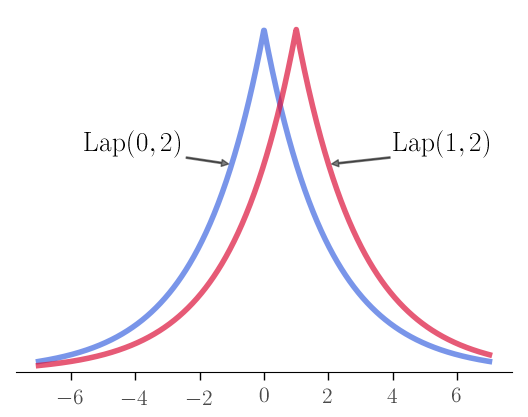
\includegraphics[width=\linewidth]{laplace}
\caption{Example of a Laplace distributions offering .5-differential privacy for
a function with sensitivity 1.} \label{fig:laplace} \end{marginfigure}

\textbf{Local differential privacy} refers to applying a privacy mechanism
locally before sending data to a centralized server. This is relevant for
collecting telemetry or data from client-side devices or browsers. Both
Apple \cite{apple-local-differential-privacy} and Google
\cite{erlingsson2014rappor} developed locally private systems for data
collection.

Differential privacy academic literature tends to be oriented to one-shot
releases of data, like the US Census, or a fixed set of database queries. In
practice, these mechanisms may be difficult to apply to fast-changing databases,
data with adversarial inputs, or unbounded numbers of queries.

\section{Synthetic Data}

\textbf{Synthetic data} involves taking real data and generating fake data sets
that preserve statistical properties. Machine learning models trained on real
data points can often be used to also generate sets of realistic-looking
synthetic data. There are risks that unintentionally memorized data
\cite{DBLP:journals/corr/abs-1802-08232} embedded in machine learning models
could be output in synthetic data sets. Because of this risk, differential
privacy is often coupled with synthetic data generation to ensure that output is
private. NIST recently ran a contest for generating such differentially private
synthetic data sets \cite{nist-synthetic-data}.

\section{Secure Enclaves}

\textbf{Secure enclaves} are a CPU technology that provide a safe place to run
code and perform computations on an otherwise unsafe platform. Intel Software
Guard Extensions (SGX) \cite{intel-sgx} is one example of a more widely
available enclave technology. In the context of privacy, enclaves allow one
party (e.g. a regulator) to compute over another party’s private data (e.g. a
service provider) without learning any of the service provider’s data.
Furthermore, the service provider would not be able to know what a regulator is
even searching for.

SGX is the basis for multiple privacy-preserving machine learning schemes
\cite{DBLP:conf/eurosp/ChengZKHHJJ0S19,tramer2018slalom,DBLP:journals/corr/abs-1803-05961}.
The biggest barriers to adoption at this time is the availability of SGX in
deployed servers and the lack of experience in enclave development by most
parties. SGX is available on Microsoft Azure under the name Confidential
Computing \cite{azure-confidential-computing}.  Microsoft is also making
software tools available a part of the new Confidential Computing Consortium.
Google also developed a privacy analytics tool, Prochlo \cite{prochlo}, based on
SGX.

\section{Mix Networks}

\textbf{Mix networks} \cite{DBLP:journals/cacm/Chaum81} are protocols between
mutually distrustful parties to shuffle values and unlink values from inputer’s
identities. Tor is the most well known mix net used practice and is intended to
unlink someone's source IP address from destination IP addresses
\cite{DBLP:conf/uss/DingledineMS04}. Mix nets also are often proposed in voting
schemes to anonymously shuffle votes.

\begin{marginfigure} 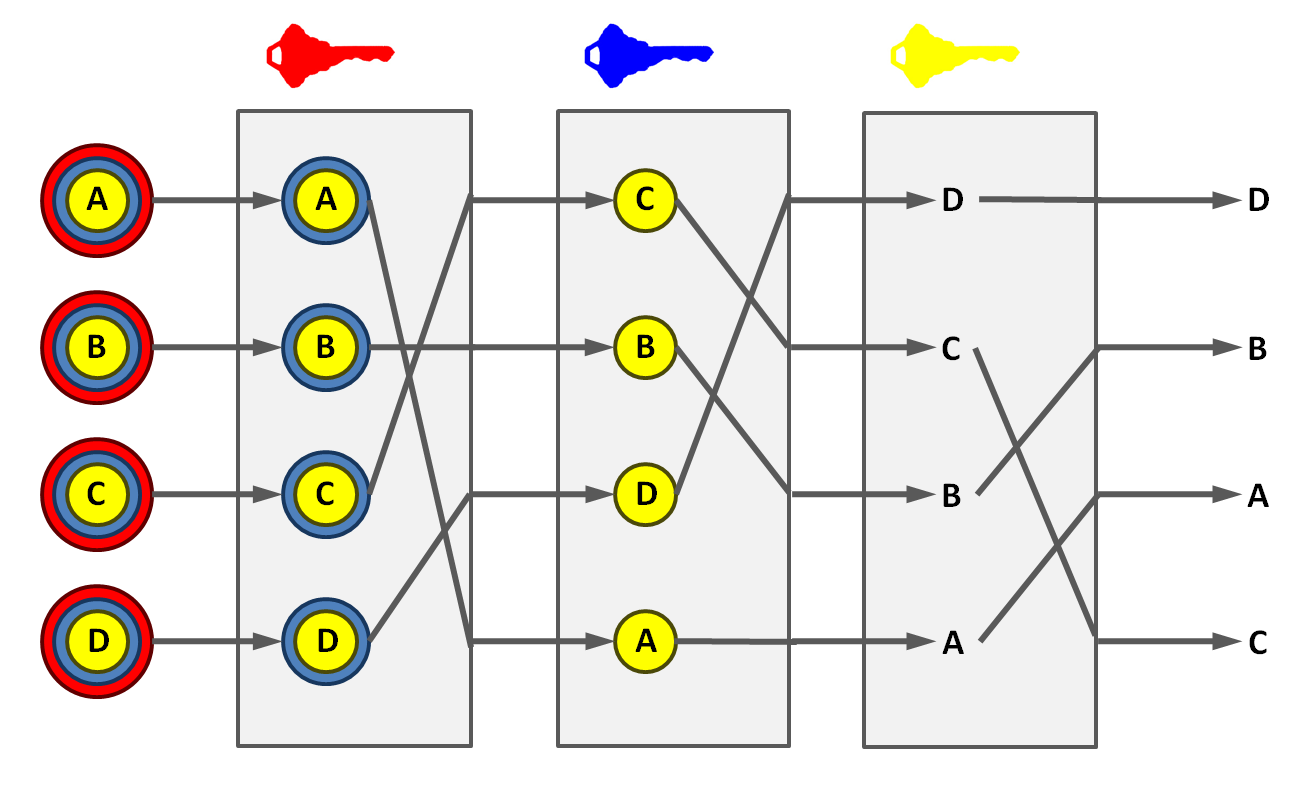
\includegraphics[width=\linewidth]{mixnet}
\caption{An example decryption mixnet between three parties. Each message is
encrypted by a sequences of public keys. Each party in the mixnet removes one
layer by decrypting using its own key then outputs messages in a random order.}
\label{fig:mixnet} \end{marginfigure}

In the scope of data sharing, mix networks can be used as a tool to allow third
parties to unlink individual identities from data sets. For example, a similar
concept of a “mix zone” was proposed as a way
 of achieving $k$-anonymity of
transit trajectories \cite{freudiger2007mix}.

\section{Advanced Cryptography}

Cryptography offers multiple technologies for privately computing over data,
including secure \textbf{multiparty computation} (MPC), \textbf{homomorphic
encryption}, or \textbf{functional encryption}. These techniques are generall
too slow for large scale applications and have not been standardized into common
tools. There are few examples of practical deployments for data privacy, though
more companies are working on this space.

The most practical applications tend to be hybrid and combine secure enclaves
for performance-sensitive operations. One exception may be Google’s work on
\textbf{Private Set Intersection}, which is likely being used to join ad click
data with Mastercard’s purchase data. This is fairly limited and is just for
summing common values between two parties’ data sets.

\section{Verifiable Data \& Verifiable Computation}

An underlying motivation for data sharing is that one party may not trust
another to report honest aggregate data. For example, regulatory agencies
conducting oversight may not trust aggregate data from service providers.
\textbf{Verifiable data structures} allow parties to verify whether an element
is a member of a set and, in some cases, whether it is a non-member. Google’s
Trillian verifiable data structures are used by Certificate Transparency (CT) to
allow browsers to verify whether a TLS certificate is a member of a known set.
CT functions as a publicly verifiable, immutable log similar to a blockchain,
except for being permissioned.

The regulator use case would require a service provider to prove that they
accurately computed over private data. Zero knowledge proofs are a building
block to prove knowledge of some value without revealing what it is. In
practice, zk-SNARKs are one tool used to prove that anonymous digital currency
transactions sum to the correct values. zk-SNARKs are used to prove that a
transaction isn’t creating or destroying money without revealing who is getting
paid or how much.

The combination of a verifiable data structure and zero knowledge proof system
could allow a regulator to verify data provided by a service probvider. It would
work by having a service provider commit to a log of ciphertexts or oblivious
committments before sharing aggregated data. Then the service provider could
prove that the inputs to the data aggregation correspond to the committed
values. An analog of this are verifiable voting schemes where secret commitments
to votes are published, privately tallied, then available for audit to third
parties.

\bibliography{priv-mech} \bibliographystyle{acm}

\end{document}
